\section{Generating contention via DMA}
\label{sec:interconnect-sc-dma}

We now move on to the case of detecting memory contention using direct memory access (DMA) transfers.
We revisit \textbf{RQ1} to determine if an adversary can use this approach to observe the victim's traffic pattern. 
In addition, we also provide an answer to \textbf{RQ2} by demonstrating that an adversary can create congestion on a non-hierarchical PCIe 4.0 link.

A DMA controller can generate memory addresses and initiate memory \textit{load} or \textit{store} instructions that are executed in parallel, independent of the execution units of the CPU.
The DMA controller receives commands specifying the source and destination addresses and the size of the data to copy.
Once the data transfer is complete, it issues a notification of completion to the command issuer.
As such, DMA controllers such as those on Nvidia GPUs provide a mechanism to measure only the completion time of the entire DMA transfer, not the completion time of individual \textit{load} or \textit{store} instructions.

\subsection{Challenges}
\label{subsec:interconnect-sc-dma-challenges}
\subsection{Using DMA operations to observe presence/absence of victim traffic on PCIe}
\label{subsec:interconnect-sc-dma-evaluation}

Now that we know that the PCIe bandwidth can be saturated with 4MB transfers, we can use this information to craft an adversary that can create congestion in the non-hierarchical PCIe link.
To achieve this, we use the pseudo-code outlined in \Cref{lst:timing-victim-with-dma}.
We assume that the victim is also transferring data to/from the GPU via DMA.

To evaluate our ability to detect victim traffic, we run the adversary for $10^4$ iterations.
At the same time, we execute the victim, which repeatedly (for $10^3$ iterations) performs a DMA transfer of either 4KB or 4MB
As before, we synchronise the execution of the critical code sections responsible for data transfers between the victim and the adversary. 

As shown in \Cref{fig:dma-contention-4mb}, the time it takes to complete the call to \textit{cudaMemcpy} increases in the presence of victim traffic and reduces once the victim stops transmitting.
As such, an adversary is able to determine the presence/absence of victim traffic.

We also explore if the adversary can determine this without saturating the PCIe bandwidth.
For this, we follow the same pseudo-code in \Cref{lst:timing-victim-with-dma}, but set the transfer size of the adversary to 4KB.
As shown in \Cref{fig:dma-contention-4kb}, the adversary can still observe the presence or absence of the victim traffic.

\begin{minipage}{\textwidth}
    \lstinputlisting[language=Python]{code/interconnect-sc/timing-victim-with-dma.py}
    \captionsetup{type=lstlisting}
    \caption{Attacker code to detect presence of victim traffic via DMA operations}
    \label{lst:timing-victim-with-dma}
\end{minipage}

\begin{figure}
     \centering
     
     \begin{subfigure}[b]{\textwidth}
        \centering
        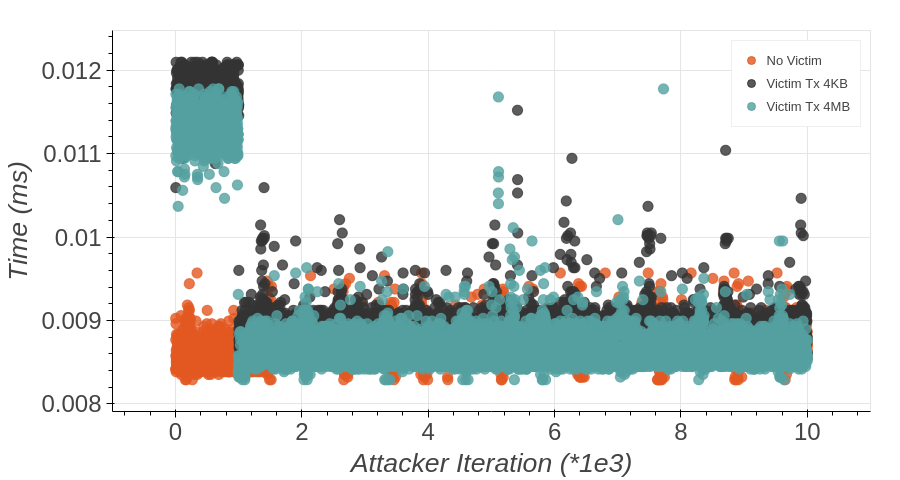
\includegraphics[width=\textwidth]{figures/interconnect-sc/dma/dma_contention_4KB.png}
        \caption{Attacker transfers 4KB}
        \label{fig:dma-contention-4kb}
     \end{subfigure}
     
     \hfill
     
     \begin{subfigure}[b]{\textwidth}
         \centering
        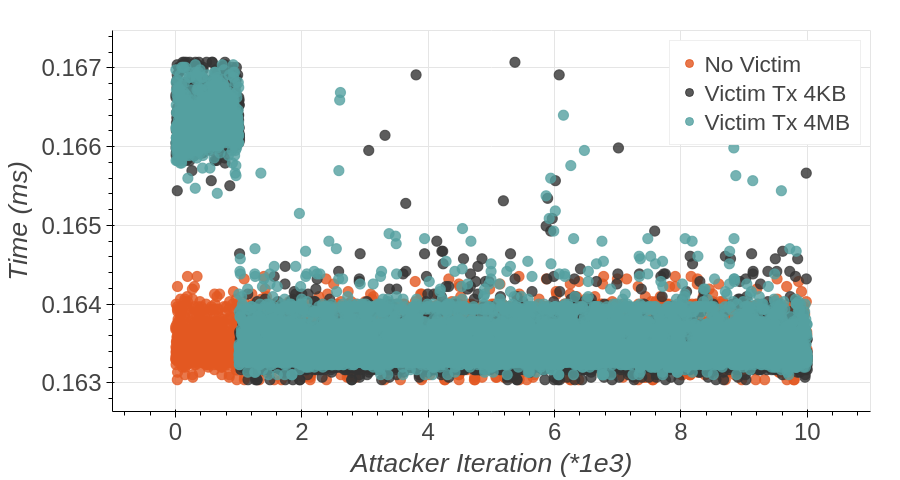
\includegraphics[width=\textwidth]{figures/interconnect-sc/dma/dma_contention_4MB.png}
        \caption{Attacker transfers 4MB}
        \label{fig:dma-contention-4mb}
     \end{subfigure}
     
    \caption{Observing the presence of victim DMA traffic using DMA operations. The victim does $10^3$ iterations of transferring 4KB/4MB.}
    \label{fig:dma-contention}
    % 2025-03-06_17-18
\end{figure}

